\documentclass[journal,12pt,twocolumn]{IEEEtran}
%
\usepackage{setspace}
\usepackage{gensymb}
\usepackage{xcolor}
\usepackage{caption}
%\usepackage{subcaption}
%\doublespacing
\singlespacing

%\usepackage{graphicx}
%\usepackage{amssymb}
%\usepackage{relsize}
\usepackage[cmex10]{amsmath}
\usepackage{mathtools}
%\usepackage{amsthm}
%\interdisplaylinepenalty=2500
%\savesymbol{iint}
%\usepackage{txfonts}
%\restoresymbol{TXF}{iint}
%\usepackage{wasysym}
\usepackage{hyperref}
\usepackage{amsthm}
\usepackage{mathrsfs}
\usepackage{txfonts}
\usepackage{stfloats}
\usepackage{cite}
\usepackage{cases}
\usepackage{subfig}
%\usepackage{xtab}
\usepackage{longtable}
\usepackage{multirow}
%\usepackage{algorithm}
%\usepackage{algpseudocode}
%\usepackage{enumerate}
\usepackage{enumitem}
\usepackage{mathtools}
%\usepackage{iithtlc}
%\usepackage[framemethod=tikz]{mdframed}
\usepackage{listings}
\let\vec\mathbf


%\usepackage{stmaryrd}


%\usepackage{wasysym}
%\newcounter{MYtempeqncnt}
\DeclareMathOperator*{\Res}{Res}
%\renewcommand{\baselinestretch}{2}
\renewcommand\thesection{\arabic{section}}
\renewcommand\thesubsection{\thesection.\arabic{subsection}}
\renewcommand\thesubsubsection{\thesubsection.\arabic{subsubsection}}

\renewcommand\thesectiondis{\arabic{section}}
\renewcommand\thesubsectiondis{\thesectiondis.\arabic{subsection}}
\renewcommand\thesubsubsectiondis{\thesubsectiondis.\arabic{subsubsection}}

%\renewcommand{\labelenumi}{\textbf{\theenumi}}
%\renewcommand{\theenumi}{P.\arabic{enumi}}

% correct bad hyphenation here
\hyphenation{op-tical net-works semi-conduc-tor}

\lstset{
	language=Python,
	frame=single, 
	breaklines=true,
	columns=fullflexible
}



\begin{document}
	%
	
	\theoremstyle{definition}
	\newtheorem{theorem}{Theorem}[section]
	\newtheorem{problem}{Problem}
	\newtheorem{proposition}{Proposition}[section]
	\newtheorem{lemma}{Lemma}[section]
	\newtheorem{corollary}[theorem]{Corollary}
	\newtheorem{example}{Example}[section]
	\newtheorem{definition}{Definition}[section]
	%\newtheorem{algorithm}{Algorithm}[section]
	%\newtheorem{cor}{Corollary}
	\newcommand{\BEQA}{\begin{eqnarray}}
		\newcommand{\EEQA}{\end{eqnarray}}
	\newcommand{\define}{\stackrel{\triangle}{=}}
	\newcommand{\myvec}[1]{\ensuremath{\begin{pmatrix}#1\end{pmatrix}}}
	\newcommand{\mydet}[1]{\ensuremath{\begin{vmatrix}#1\end{vmatrix}}}
	
	\bibliographystyle{IEEEtran}
	%\bibliographystyle{ieeetr}
	
	\providecommand{\nCr}[2]{\,^{#1}C_{#2}} % nCr
	\providecommand{\nPr}[2]{\,^{#1}P_{#2}} % nPr
	\providecommand{\mbf}{\mathbf}
	\providecommand{\pr}[1]{\ensuremath{\Pr\left(#1\right)}}
	\providecommand{\qfunc}[1]{\ensuremath{Q\left(#1\right)}}
	\providecommand{\sbrak}[1]{\ensuremath{{}\left[#1\right]}}
	\providecommand{\lsbrak}[1]{\ensuremath{{}\left[#1\right.}}
	\providecommand{\rsbrak}[1]{\ensuremath{{}\left.#1\right]}}
	\providecommand{\brak}[1]{\ensuremath{\left(#1\right)}}
	\providecommand{\lbrak}[1]{\ensuremath{\left(#1\right.}}
	\providecommand{\rbrak}[1]{\ensuremath{\left.#1\right)}}
	\providecommand{\cbrak}[1]{\ensuremath{\left\{#1\right\}}}
	\providecommand{\lcbrak}[1]{\ensuremath{\left\{#1\right.}}
	\providecommand{\rcbrak}[1]{\ensuremath{\left.#1\right\}}}
	\theoremstyle{remark}
	\newtheorem{rem}{Remark}
	\newcommand{\sgn}{\mathop{\mathrm{sgn}}}
	\providecommand{\abs}[1]{\left\vert#1\right\vert}
	\providecommand{\res}[1]{\Res\displaylimits_{#1}} 
	\providecommand{\norm}[1]{\lVert#1\rVert}
	\providecommand{\mtx}[1]{\mathbf{#1}}
	\providecommand{\mean}[1]{E\left[ #1 \right]}
	\providecommand{\fourier}{\overset{\mathcal{F}}{ \rightleftharpoons}}
	\providecommand{\ztrans}{\overset{\mathcal{Z}}{ \rightleftharpoons}}
	
	%\providecommand{\hilbert}{\overset{\mathcal{H}}{ \rightleftharpoons}}
	\providecommand{\system}{\overset{\mathcal{H}}{ \longleftrightarrow}}
	%\newcommand{\solution}[2]{\textbf{Solution:}{#1}}
	\newcommand{\solution}{\noindent \textbf{Solution: }}
	\providecommand{\dec}[2]{\ensuremath{\overset{#1}{\underset{#2}{\gtrless}}}}
	\numberwithin{equation}{section}
	%\numberwithin{equation}{subsection}
	%\numberwithin{problem}{subsection}
	%\numberwithin{definition}{subsection}
	\makeatletter
	\@addtoreset{figure}{problem}
	\makeatother
	
	\let\StandardTheFigure\thefigure
	%\renewcommand{\thefigure}{\theproblem.\arabic{figure}}
	\renewcommand{\thefigure}{\theproblem}
	
	
	%\numberwithin{figure}{subsection}
	
	\def\putbox#1#2#3{\makebox[0in][l]{\makebox[#1][l]{}\raisebox{\baselineskip}[0in][0in]{\raisebox{#2}[0in][0in]{#3}}}}
	\def\rightbox#1{\makebox[0in][r]{#1}}
	\def\centbox#1{\makebox[0in]{#1}}
	\def\topbox#1{\raisebox{-\baselineskip}[0in][0in]{#1}}
	\def\midbox#1{\raisebox{-0.5\baselineskip}[0in][0in]{#1}}
	
	\vspace{3cm}
	
	\title{ 
		%\logo{
			%}
		Pingala Series
		%	\logo{Octave for Math Computing }
	}
	%\title{
		%	\logo{Matrix Analysis through Octave}{\begin{center}\includegraphics[scale=.24]{tlc}\end{center}}{}{HAMDSP}
		%}
	
	
	% paper title
	% can use linebreaks \\ within to get better formatting as desired
	%\title{Matrix Analysis through Octave}
	%
	%
	% author names and IEEE memberships
	% note positions of commas and nonbreaking spaces ( ~ ) LaTeX will not break
	% a structure at a ~ so this keeps an author's name from being broken across
	% two lines.
	% use \thanks{} to gain access to the first footnote area
	% a separate \thanks must be used for each paragraph as LaTeX2e's \thanks
	% was not built to handle multiple paragraphs
	%
	
	\author{ Aakash Kamuju$^{*}$ %<-this  stops a space
	}% <-this % stops a space
	%\thanks{J. Doe and J. Doe are with Anonymous University.}% <-this % stops a space
	%\thanks{Manuscript received April 19, 2005; revised January 11, 2007.}}
% note the % following the last \IEEEmembership and also \thanks - 
% these prevent an unwanted space from occurring between the last author name
% and the end of the author line. i.e., if you had this:
% 
% \author{....lastname \thanks{...} \thanks{...} }
%                     ^------------^------------^----Do not want these spaces!
%
% a space would be appended to the last name and could cause every name on that
% line to be shifted left slightly. This is one of those "LaTeX things". For
% instance, "\textbf{A} \textbf{B}" will typeset as "A B" not "AB". To get
% "AB" then you have to do: "\textbf{A}\textbf{B}"
% \thanks is no different in this regard, so shield the last } of each \thanks
% that ends a line with a % and do not let a space in before the next \thanks.
% Spaces after \IEEEmembership other than the last one are OK (and needed) as
% you are supposed to have spaces between the names. For what it is worth,
% this is a minor point as most people would not even notice if the said evil
% space somehow managed to creep in.



% The paper headers
%\markboth{Journal of \LaTeX\ Class Files,~Vol.~6, No.~1, January~2007}%
%{Shell \MakeLowercase{\textit{et al.}}: Bare Demo of IEEEtran.cls for Journals}
% The only time the second header will appear is for the odd numbered pages
% after the title page when using the twoside option.
% 
% *** Note that you probably will NOT want to include the author's ***
% *** name in the headers of peer review papers.                   ***
% You can use \ifCLASSOPTIONpeerreview for conditional compilation here if
% you desire.




% If you want to put a publisher's ID mark on the page you can do it like
% this:
%\IEEEpubid{0000--0000/00\$00.00~\copyright~2007 IEEE}
% Remember, if you use this you must call \IEEEpubidadjcol in the second
% column for its text to clear the IEEEpubid mark.



% make the title area
\maketitle

%\newpage

\tableofcontents

%\renewcommand{\thefigure}{\thesection.\theenumi}
%\renewcommand{\thetable}{\thesection.\theenumi}

\renewcommand{\thefigure}{\theenumi}
\renewcommand{\thetable}{\theenumi}

%\renewcommand{\theequation}{\thesection}


\bigskip

\begin{abstract}
This manual provides a simple introduction to Transforms
\end{abstract}
\section{JEE 2019}
Let 
\begin{align}
a_n &= \frac{\alpha^{n}-\beta^{n}}{\alpha - \beta}, \quad n \ge 1
\\
b_n &= a_{n-1} + a_{n+1}, \quad n \ge 2, \quad b_1 =1
\label{eq:10-orig-diff}
\end{align}
Verify the following using a python code.
\begin{enumerate}[label=\thesection.\arabic*
,ref=\thesection.\theenumi]
\item 
\begin{align}
	\sum_{k=1}^{n}a_k = a_{n+2}-1, \quad n \ge 1
\end{align}
\solution:
Run the below python code 
\begin{lstlisting}
	wget https://github.com/kamujuaakash/EE3900/blob/main/pingala/codes/1.py
\end{lstlisting}
Use the following command in the terminal to run the code
\begin{lstlisting}
	python3 1.py
\end{lstlisting}
\begin{figure}[h]
	\centering
	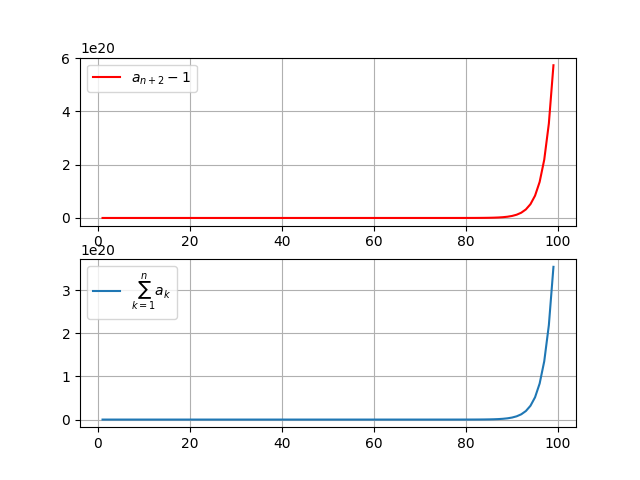
\includegraphics[width=0.7\columnwidth]{./figs/1_1.png}
	\caption{}
\end{figure}
\item 
\begin{align}
	\sum_{k=1}^{\infty}\frac{a_k}{10^k} =\frac{10}{89}
\end{align}
\solution:
Run the below python code 
\begin{lstlisting}
	wget https://github.com/kamujuaakash/EE3900/blob/main/pingala/codes/1.py
\end{lstlisting}
Use the following command in the terminal to run the code
\begin{lstlisting}
	python3 1.py
\end{lstlisting}
\begin{figure}[h]
	\centering
	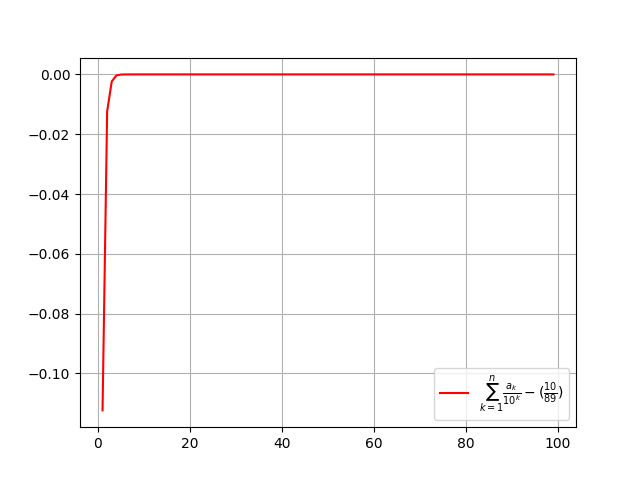
\includegraphics[width=0.7\columnwidth]{./figs/1_2.png}
	\caption{}
\end{figure}
\item 
\begin{align}
	b_n =\alpha^n + \beta^n, \quad n \ge 1
\end{align}
\solution:
Run the below python code 
\begin{lstlisting}
	wget https://github.com/kamujuaakash/EE3900/blob/main/pingala/codes/1.py
\end{lstlisting}
Use the following command in the terminal to run the code
\begin{lstlisting}
	python3 1.py
\end{lstlisting}
\begin{figure}[h]
	\centering
	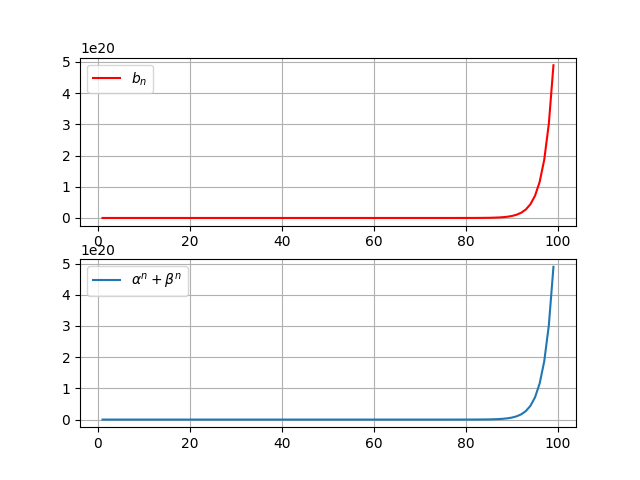
\includegraphics[width=0.7\columnwidth]{./figs/1_3.png}
	\caption{}
\end{figure}
\item 
\begin{align}
	\sum_{k=1}^{\infty}\frac{b_k}{10^k} =\frac{8}{89}
\end{align}
\solution:
Run the below python code 
\begin{lstlisting}
	wget https://github.com/kamujuaakash/EE3900/blob/main/pingala/codes/1.py
\end{lstlisting}
Use the following command in the terminal to run the code
\begin{lstlisting}
	python3 1.py
\end{lstlisting}
\begin{figure}[h]
	\centering
	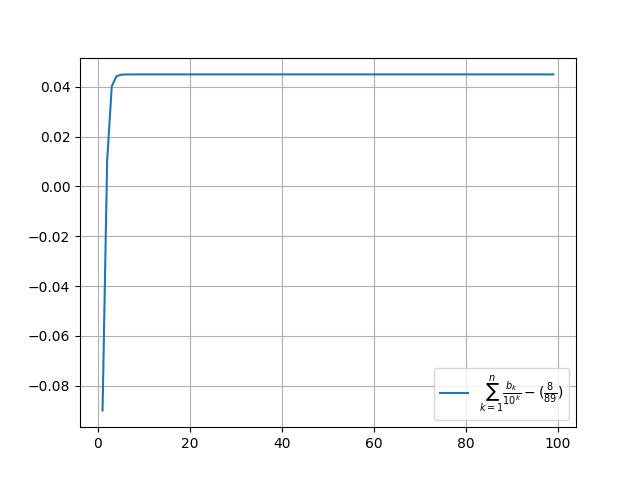
\includegraphics[width=0.7\columnwidth]{./figs/1_4.png}
	\caption{}
\end{figure}
Clearly from the figure this isnt true, it actually converges to $\frac{12}{89}$
\end{enumerate}
\section{Pingala Series}
\begin{enumerate}[label=\thesection.\arabic*,ref=\thesection.\theenumi]
\item The {\em one sided} $Z$-transform of $x(n)$ is defined as 
%\cite{proakis_dsp}
\begin{align}
	X^{+}(z) = \sum_{n = 0}^{\infty}x(n)z^{-n}, \quad z \in \mathbb{C}
	\label{eq:one-Z}
\end{align}
\item The {\em Pingala} series is generated using the difference equation 
\begin{align*}
	x(n+2) = x\brak{n+1} + x\brak{n}\\
	x(0) = x(1) = 1, n \ge 0
	\label{eq:10-pingala}
\end{align*}
Generate a stem plot for $x(n)$.\\
\solution
Run the below python code 
\begin{lstlisting}
	wget https://github.com/kamujuaakash/EE3900/blob/main/pingala/codes/2.py
\end{lstlisting}
Use the following command in the terminal to run the code
\begin{lstlisting}
	python3 2.py
\end{lstlisting}
\begin{figure}[ht!]
	\centering
	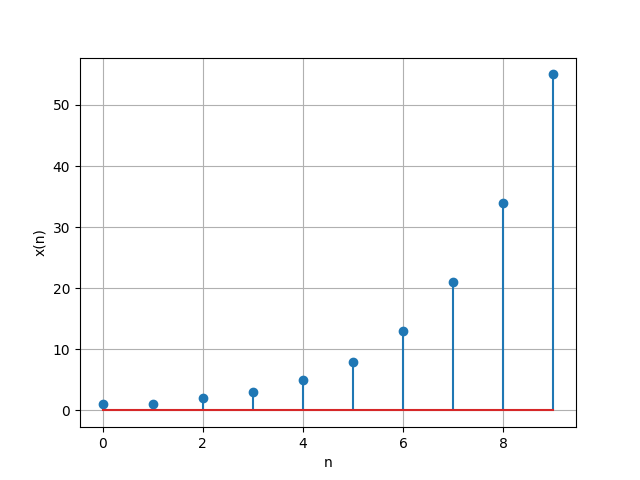
\includegraphics[width=\columnwidth]{./figs/2_2.png}
	\caption{}
\end{figure}
\item Find $X^{+}(z)$.\\
\solution:
\begin{align}
	x(n+2) = x\brak{n+1} + x\brak{n}
\end{align}
applying positive Z-transform on both sides,also wkt it is a linear operator
\begin{align}
	&\sum_{k=0}^{\infty}x(k+2)z^{-k}=\sum_{k=0}^{\infty}x(k+1)z^{-k}+\sum_{k=0}^{\infty}x(k)z^{-k}\\
	&z^{2}(X^{+}(z)-x(0)-x(1)z^{-1})=X^{+}(z)+z(X^{+}(z)-x(0))\\
	&\implies X^{+}(z)=\frac{z^{2}}{z^{2}-z-1}\\
	&\implies X^{+}(z)=\frac{1}{1-z^{-1}-z^{-2}}
\end{align}
\item Find $x(n)$.\\
\solution:
\begin{equation}
	X^{+}(z)=\frac{1}{(1-\alpha z^{-1})(1-\beta z^{-1})}
\end{equation}
where $\alpha,\beta$ are the roots of equation
\begin{equation}
	z^2-z-1=0
\end{equation}
coefficient of $z^{-k}$ in the above expression is $x(k)$ by comparing LHS and RHS\\
\begin{equation}
	X^{+}(z)=\frac{1}{\alpha-\beta}\left(\frac{\alpha}{1-\alpha z^{-1}}-\frac{\beta}{1-\beta z^{-1}}\right)
\end{equation}
$\therefore$ using binomial theorem we get
\begin{equation} 
	x(k)=\frac{\alpha^{k+1}-\beta^{k+1}}{\alpha - \beta}
\end{equation}
\item Sketch 
\begin{align}
	y(n)	 = x\brak{n-1} + x\brak{n+1},  \quad n \ge 0
\end{align}
\solution
Run the below python code 
\begin{lstlisting}
	wget https://github.com/kamujuaakash/EE3900/blob/main/pingala/codes/2.py
\end{lstlisting}
Use the following command in the terminal to run the code
\begin{lstlisting}
	python3 2.py
\end{lstlisting}
\begin{figure}[h]
	\centering
	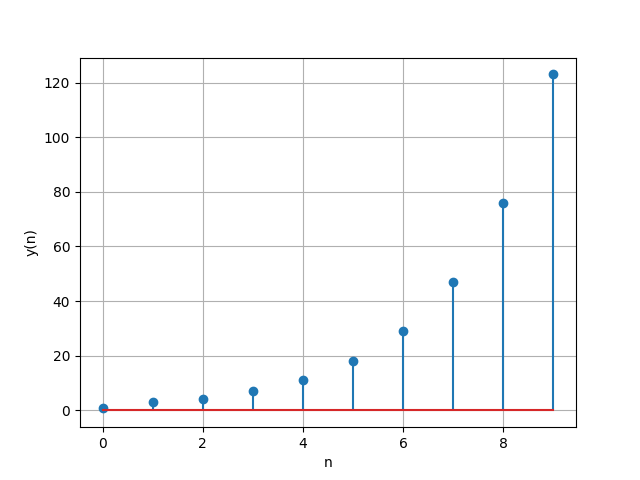
\includegraphics[width=\columnwidth]{./figs/2_5.png}
	\caption{}
\end{figure}
\item Find $Y^{+}(z)$.
\\
\solution:
Taking +ve Z-transform on both sides of equation 
\begin{align}
	&\sum_{k=0}^{\infty}y(k)z^{-k}=\sum_{k=0}^{\infty}x(k+1)z^{-k}+\sum_{k=0}^{\infty}x(k-1)z^{-k}\\
	&Y^{+}(z)=z(X^{+}(z)-x(0))+z^{-1}X^{+}(z)\\
	&\because x(-1)=0 \nonumber \\
	&Y^{+}(z)=\frac{z+z^{-1}}{1-z^{-1}-z^{-2}}-z\\
	&\therefore Y^{+}(z)=\frac{1+2z^{-1}}{1-z^{-1}-z^{-2}}
\end{align}
\item Find $y(n)$.\\
\solution:
Coefficient of $z^{-n}$ in $Y^{+}(z)$ will be $y(n)$
\begin{align}
	&Y^{+}(z)=\frac{1}{1-z^{-1}-z^{-2}}+\frac{2z^{-1}}{1-z^{-1}-z^{-2}}\\
	&y(k)=\frac{\alpha^{k+1}-\beta^{k+1}}{\alpha - \beta} +2\frac{\alpha^{k}-\beta^{k}}{\alpha - \beta}\\
	&=\frac{\alpha^{k+2}+\alpha^{k}-\beta^{k}-\beta^{k+2}}{\alpha-\beta}\\
	&=\frac{\alpha^{k+2}-\beta^{k+2}+\alpha \beta^{k+1}-\beta \alpha^{k+1}}{\alpha-\beta} [\because \alpha \beta=-1]\\
	&\therefore y(k)=\alpha^{k+1}+\beta^{k+1}
\end{align}
\end{enumerate}
\section{Power of the Z transform}
\begin{enumerate}[label=\thesection.\arabic*,ref=\thesection.\theenumi]
\item Show that 
\begin{align}
	\sum_{k=1}^{n}a_k = 
	\sum_{k=0}^{n-1}x(k) = x(n)*u(n-1)
\end{align}
\solution:
\begin{align}
	& x(k)=a(k+1)\\
	&\implies \sum_{k=0}^{n-1} x(k)=\sum_{k=0}^{n-1} a(k+1)\\
	&\implies \sum_{k=1}^{n}a_{k} = \sum_{k=0}^{n-1}x(k)\\
	& x(n)*u(n-1)=\sum_{k=-\infty}^{\infty} x(k) u(n-1-k)\\
	&u(n-1-k)=\begin{cases}
		0 & k>n-1\\
		1 & k>=n-1
	\end{cases}\\
	&x(k)=0 \forall k<0\\
	&\therefore x(n)*u(n-1)=\sum_{k=0}^{n-1} x(k)
\end{align}
\item Show that 
\begin{align}
	a_{n+2}-1, \quad n \ge 1
\end{align}
can be expressed as 
\begin{align}
	\sbrak{x\brak{n+1}-1}u\brak{n}
\end{align}
\solution:
\begin{align}
	&x(k)=a(k+1)\\
	&\implies x(k+1)=a(k+2)\\
	&a(k+2)-1=x(k+1)-1\\
	&\therefore =[x(k+1)-1]u(k)[\because \forall n>=1]
\end{align}
\item Show that 
\begin{align}
	\sum_{k=1}^{\infty}\frac{a_k}{10^k}= 
	\frac{1}{10}\sum_{k=0}^{\infty}\frac{x\brak{k}}{10^k} =\frac{1}{10}X^{+}\brak{{10}}
\end{align}
\solution:
\begin{align}
	&X^{+}(z)=\sum_{k=0}^{\infty} x(k)z^{-k}=z\sum_{k=1}^{\infty} a(k) z^{-k}\\
	&z=10\\
	&\implies 10\sum_{k=1}^{\infty}\frac{a_k}{10^k}=\sum_{k=0}^{\infty}\frac{x\brak{k}}{10^k} =X^{+}\brak{{10}}\\
	&\implies \sum_{k=1}^{\infty}\frac{a_k}{10^k}= 
	\frac{1}{10}\sum_{k=0}^{\infty}\frac{x\brak{k}}{10^k} =\frac{1}{10}X^{+}\brak{{10}}
\end{align}
\item Show that 
\begin{align}
	\alpha^n + \beta^n, \quad n \ge 1
\end{align}
can be expressed as 
\begin{align}
	w(n) =\brak{\alpha^{n+1} + \beta^{n+1}}u(n)
\end{align}
and find $W(z)$.\\
\solution:
applying Z-transform on both sides,
\begin{align}
	&W(z)=\sum_{n=-\infty}^{\infty}\brak{\alpha^{n+1} + \beta^{n+1}}u(n)z^{-n}\\
	&=\sum_{n=0}^{\infty}\brak{\alpha^{n+1} + \beta^{n+1}}z^{-n}\\
	&=\alpha \sum_{n=0}^{\infty}(\alpha z^{-1})^{n}+\beta \sum_{n=0}^{\infty} (\beta z^{-1})^{n}\\
	&\text{ROC:} |z|>\text{max}(\alpha,\beta)\\
	&=\frac{\alpha}{1-\alpha z^{-1}}+\frac{\beta}{1-\beta z^{-1}}\\
	&=\frac{1+2z^{-1}}{1-z^{-1}-z^{-2}}
\end{align}
\item Show that 
\begin{align}
	\sum_{k=1}^{\infty}\frac{b_k}{10^k} =
	\frac{1}{10}\sum_{k=0}^{\infty}\frac{y\brak{k}}{10^k} =\frac{1}{10}Y^{+}\brak{{10}}
\end{align}
\solution:
\begin{align}
	&y(k)=b(k+1)\\
	&\sum_{k=0}^{\infty} y(k) z^{-k}=\sum_{k=0}^{\infty} b(k+1) z^{-k}=Y^{+}(z)\\
	&\sum_{k=0}^{\infty} y(k) z^{-k}=z\sum_{k=1}^{\infty} b(k) z^{-k}=Y^{+}(z)\\
	&z=10\\
	&\implies \sum_{k=1}^{\infty}\frac{b_k}{10^k} =
	\frac{1}{10}\sum_{k=0}^{\infty}\frac{y\brak{k}}{10^k} =\frac{1}{10}Y^{+}\brak{{10}}
\end{align}
\item Solve the JEE 2019 problem.\\
\solution:
\begin{align}
	&X^{+}(z)=z\sum_{k=1}^{\infty} a(k) z^{-k}=\frac{1}{1-z^{-1}-z^{-2}}\\
	&z=10\\
	&\sum_{k=1}^{\infty} \frac{a_k}{10^k}=\frac{1}{10 \left(1-\frac{1}{10}-\frac{1}{100}\right)}\\
	&=\frac{10}{89}
\end{align}
\begin{align}
	&y(k)=\alpha^{k+1}+\beta^{k+1}\\
	&y(k)=b(k+1)\\
	&\implies b(k)=\alpha^{k}+\beta^{k}
\end{align}
\begin{align}
	&\sum_{k=1}^{\infty}\frac{b_k}{10^k} =\frac{1}{10}Y^{+}\brak{{10}}\\
	&=\frac{1}{10}\left[\frac{1+\frac{2}{10}}{1-\frac{1}{10}-\frac{1}{100}}\right]\\
	&\because Y^{+}(z)=\frac{1+2z^{-1}}{1-z^{-1}-z^{-2}}\\
	&=\frac{12}{89}
\end{align}
Run the following code to get the expressions of $x(n)$ and $y(n)$
\begin{lstlisting}
	wget https://github.com/kamujuaakash/EE3900/blob/main/pingala/codes/Xk.py
\end{lstlisting}
Use the following command in the terminal to run the code
\begin{lstlisting}
	python3 Xk.py
\end{lstlisting}
\end{enumerate}
\end{document}